The main result of this paper is that we can approximate $\hbn$ very efficiently, and that this approach outperforms a more \naive approach of a typical deconvolution filter, half-wave rectified (i.e., setting everything below zero equal to zero).  Fig. \ref{fig:adam1} depicts an example. Clearly, the \foopsi filter is outperforming the optimal linear deconvolution filter (also called a Wiener filter).  The Wiener filter implicitly approximates the Poisson spike rate with a Gaussian spike rate (see Appendix for details). While a Gaussian well approximates a Poisson distribution when rates are about $10$ spikes per frame, this example is obviously very far from that regime, and so the Gaussian approximation does very poorly. Furthermore, the Gaussian approximation allows for the inferred spike train to include negative numbers, which we do not want, as spike trains are non-negative entities.  To counteract the negative values, the Wiener filter then infers large positive values, contributing to a ``ringing'' effect.  The non-negative constraint imposed by the \foopsi filter ensures that such ringing does not take place.  Furthermore, finding appropriate thresholds, to convert the inferred approximate spike train into a binary sequence, would clearly be more difficult for the Wiener filter than the \foopsi filter. Finally, by utilizing Gaussian elimination and interior-point methods, as described in the Methods section, the computational complexity of \foopsi filter is the same as an efficient implementation of the Wiener filter.  

\begin{figure}[h!]
\centering 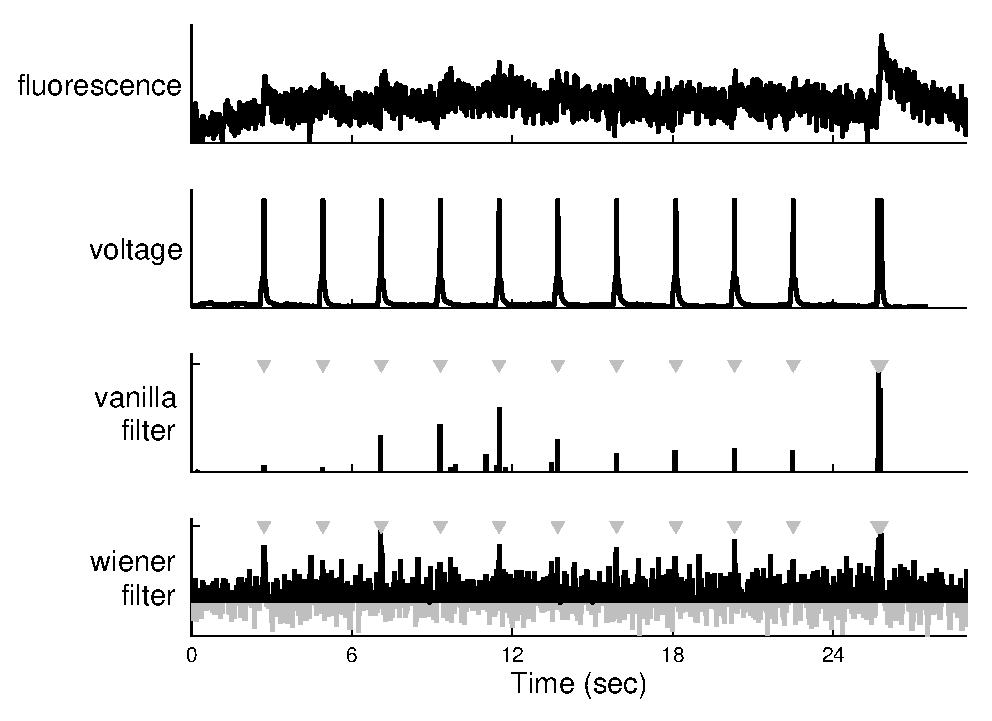
\includegraphics[width=.9\linewidth]{../figs/adam1}
\caption{The \foopsi filter significantly outperforms the optimal linear deconvolution (aka, Wiener) filter on typical simulated data-sets.  Note that all the parameters for the \foopsi filter were estimated from the data.  Simulation details: $T=2930$ time steps, $\Del=5$ msec, $\alpha=1$, $\beta=0$, $\sig=0.3$, $\tau=1$ sec, $\lam=1$ Hz.} \label{fig:woopsi}
\end{figure}

% \begin{figure}[h!]
% \centering 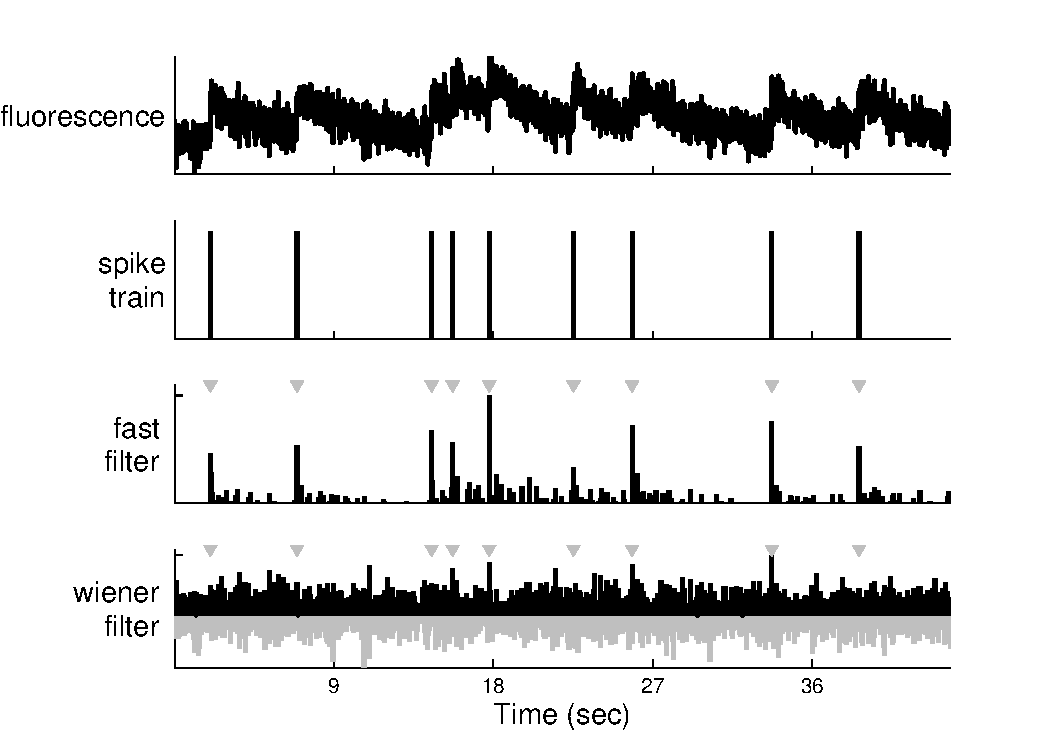
\includegraphics[width=.9\linewidth]{../figs/woopsi}
% \caption{The \foopsi filter significantly outperforms the optimal linear deconvolution (aka, Wiener) filter on typical simulated data-sets.  Note that all the parameters for the \foopsi filter were estimated from the data.  Simulation details: $T=2930$ time steps, $\Del=5$ msec, $\alpha=1$, $\beta=0$, $\sig=0.3$, $\tau=1$ sec, $\lam=1$ Hz.} \label{fig:woopsi}
% \end{figure}
% 
%in \emph{linear} time, whereas an exact solution would require exponential time. Fig. \ref{fig:wiener} shows two examples of running the \foopsi filter on simulated data.  On the left, the data is simulated according to Eqs. \eqref{eq:F} and \eqref{eq:C}, with a low expected firing rate (5 Hz).  The \foopsi filter performs very well (middle left panel): when spikes occured (gray downward facing triangles), the \foopsi filter's output is relatively high, and in the absence of a spike, the \foopsi filter's output is relatively low. The height of the ``spikes'' in $\hbn$ can be thought of as the probability of a spike having occurred.  The Wiener filter does not perform as well on this data.  Specifically, $\bn^{Wiener}$ exhibits a ``ringing'' effect, in which the inference oscillates around zero in the absence of true spikes.  This occurs because negative spikes improve the inference, if negative spikes are allowed.  By constraining our inference to be non-negative (for the \foopsi filter), we completely circumvent this problem.  
% 
% It is unsurprising that the \foopsi filter significantly outperforms the Wiener filter when spiking is sparse, given that the exponential is a much better approximation to the Poisson in this regime (c.f. Figure \ref{fig:dist_comp}).  However, even in the fast firing rate scenario, where the Gaussian approximation is far more accurate, the \foopsi filter performs relatively well, as depicted in the right panels of Figure \ref{fig:wiener}.  Note however that the computational time for computing the \foopsi filter scales linearly with $T$, i.e. is $O(T)$, whereas the \nai ve implementation of the Wiener filter requires $O(T \log T)$ (but see Appendix \ref{sec:app} for an implementation of the Wiener for that only requires $O(T)$).  
% 
% \begin{figure}[h!]
% \centering 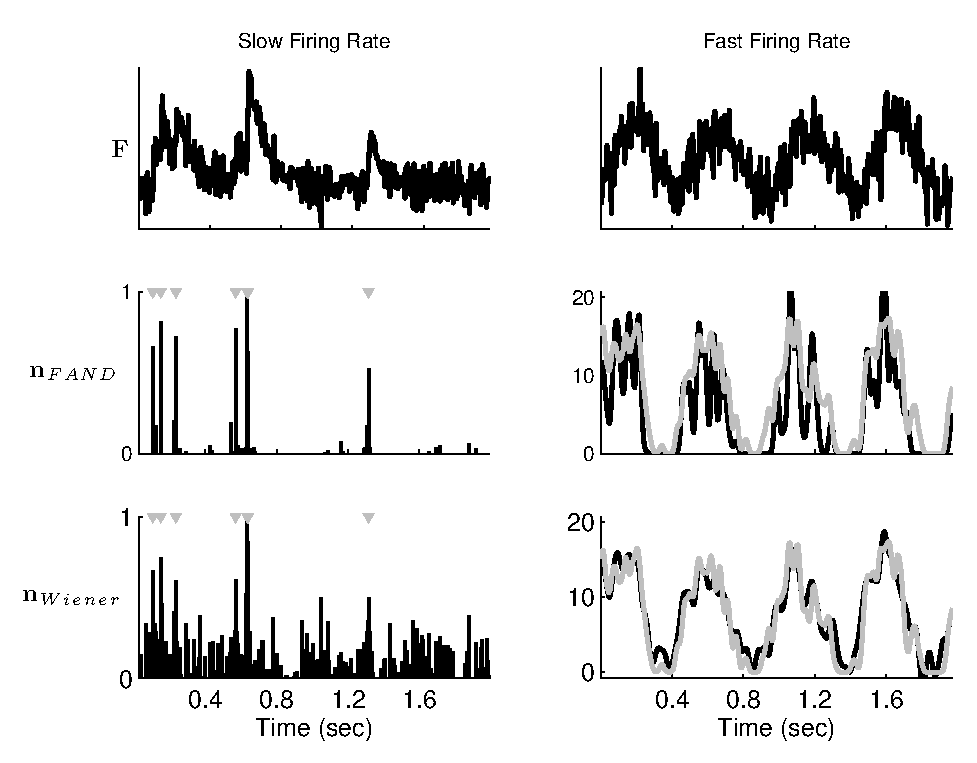
\includegraphics[width=.9\linewidth]{../figs/example_sim}
% \caption{A simulation demonstrating the performance of the \foopsi filter in different firing regimes. The left panels show that in the sparse firing regime, the \foopsi filter outperforms the Wiener filter in terms of SNR.  This follows because an exponential is a closer approximation to a Poisson than a Gaussian, when spiking is sparse. The right panels show that both approximations are good in the fast firing regime. Top left panel: fluorescence time series for a neuron with a slow firing rate.  Middle left panel: the \foopsi filter's inferred spike train.  Bottom left panel: Wiener filter's inferred spike train.  Note that (i) the Wiener filter does not impose a non-negativity constraint, and (ii) the effective SNR of the Wiener filter in this example is worse than the \foopsi filter's.  Top right panel: same as top left panel, for a neuron with a high firing rate.  Middle right panel: the \foopsi filter's inferred spike train smoothed with a Gaussian kernel for visualization purposes (black line), and the true spike train smoothed with the same Gaussian kernel (gray line).  Bottom right panel: same as middle right panel, but with the Wiener filter. Parameters for left panels: same as in Figure \ref{fig:schem}.  Parameters for right panels: same as Figure \ref{fig:schem}, except: $\sig=8$ photons, $\lam=500$ Hz.} \label{fig:wiener}
% \end{figure}
% 
% To quantify the relative quality of these inference algorithms in the sparsely spiking regime, we compute the effective signal-to-noise ratio (eSNR), defined as the average squared magnitude of the inferred spiked during frames in which there was a spike, divided by the same quantity computed in frames lacking a spike.  The left panels of Figure \ref{fig:stats} show how the eSNR varies as a function of the magnitude of the noise on observations (top left panel), and the expected firing rate (bottom left panel).  The \foopsi filter's inference (blue line) dominates the Wiener filter (red line), as well as the post-hoc half wave rectifier Wiener filter, $[$Wiener$]_+$ (green line), and a simple dF/F (turquoise line).  
% 
% When the neuron is exhibiting a high firing rate, we compute the mean-squared error (MSE) between the inferred number of spikes, and the true number of spikes.  The top right panel of Figure \ref{fig:stats} shows that when noise is relatively low, the \foopsi filter performs about as well as the Wiener filter.  However, in the high noise regime, the Wiener filter clearly outperforms the \foopsi filter.  
% 
% To verify that both our implementations of the \foopsi filter and the Wiener filter scale linear with respect to the number of image frames, the bottom right panel of Figure \ref{fig:stats} shows a such a linear relationship (on a log-log scale).  
% 
% The take home message from Figure \ref{fig:stats} is that when we expect $<1$ spike per frame, the \foopsi filter significantly outperforms the Wiener filter, regardless of variance of the observation noise.  Furthermore, because of our linear time algorithm, filtering around 50,000 image frames requires only about 1 second on a standard Apple laptop.  Below, we improve on our inference quality by generalizing our model in a number of ways.
% 
% \begin{figure}[h!]
% \centering 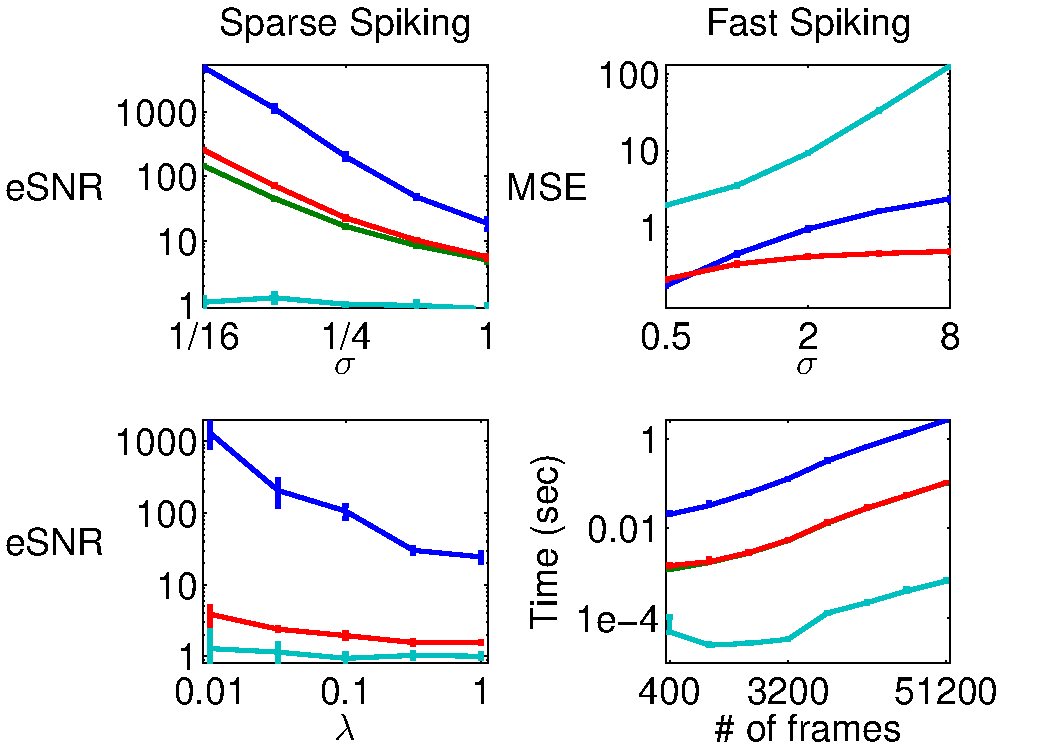
\includegraphics[width=.9\linewidth]{../figs/stats}
% \caption{Quantitative assessment of the \foopsi filter's inference quality and speed.  The left columns show that the \foopsi filter outperforms the Wiener filter in terms of eSNR --- Eq. \eqref{eq:SNR} --- regardless of variance of observation noise (top) and expected firing rate (bottom).  The top right panel show that when noise is low, even when firing rates are relatively (e.g. $\lam \Del=20$ Hz), the \foopsi filter and Wiener filter both perform well.  Both algorithms scale linearly with the number of image frames, meaning that it takes about 1 second of computational time per 50,000 image frames, using either algorithm.  Simulation details: 5 simulations for each point on all the plots, mean (solid line) and standard deviation (bars) are shown for each.  Parameters: $\Del = 0.005$ sec, $\alpha=1$, $\beta=0$.  Top left: $\lam=1$ Hz, $\tau=1$ sec.  Top right: $\lam=10$ Hz, $\tau=1$ sec.  Bottom left: $\sig=0.25$, $\tau=0.5$ sec.  Bottom right: $\sig=0.25$, $\tau=0.1$ sec, $\lam=1$ Hz.} \label{fig:stats}
% \end{figure}
% 
% Finally, often one is interested in understanding the relationship between spike trains and the environment.  Therefore, we simulated a neuron whose spiking activity was a function of a 5-dimensional external stimulus.  More specifically, we let $\lam_t = \bk\T \bx_t$, where $\bk$ is a 5-dimensional linear kernel, $\bx_t$ is the stimulus at time $t$, and $P(n_t)=$Poisson($\lam_t \Del$).  We then computed the maximum likelihood estimate of the linear kernel, $\hbk=\hbn \bx\T (\bx \bx\T)^{-1}$.  Importantly, the simulation was constructed to incorporate both sparse spiking and fast spiking periods, much like sensory neurons have periods of quiescence, followed by stimulus driven bursts.  Thus, neither the \foopsi filter nor the Wiener filter's assumptions are entirely appropriate. Figure \ref{fig:kernel} shows the results of this simulation.  The true kernel, kernel estimated using the true spike times, and kernel estimated using the \foopsi filter, are nearly overlapping (black, gray, and blue lines, respectively).  The kernel estimated using the Wiener filter output, however, is effectively flat (red line). Post-hoc half-wave rectification of the Wiener filter output does not improve its ability to estimate this kernel (green line --- completely obscured by the unrectified Wiener filter output).  Finally, dF/F does not yield anything useful at all (turquoise line).  This simulation provides further evidence of the quantitative advantage of utilizing the \foopsi filter before performing an analysis on calcium fluorescence data.
% 
% \begin{figure}[h!]
% \centering 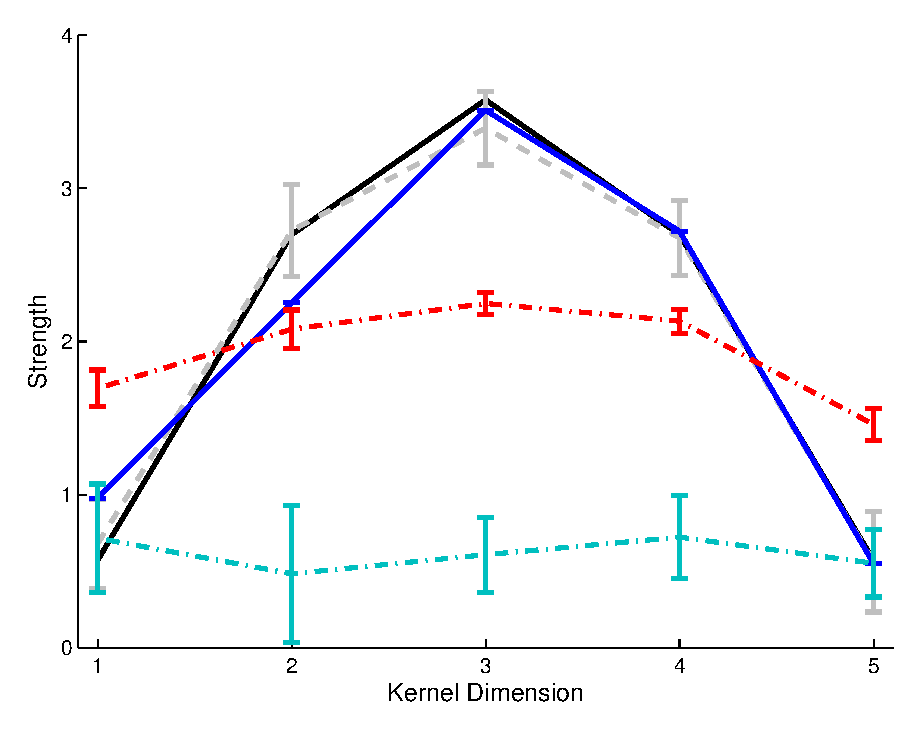
\includegraphics[width=.9\linewidth]{../figs/kernel}
% \caption{The tuning curve of a neuron (black line), estimating from the true spike train (gray line), and the inferred spike train using the (i) \foopsi filter (blue line), (ii) Wiener filter (red line), and (iii) dF/F.  Clearly, the \foopsi filter performs nearly as well as the true spike train, whereas the Wiener filter and dF/F do not.  Note that half-wave rectification of the Wiener did not change the results at all.  Simulation details: mean (solid lines) and standard deviation (bars) of 5 simulations,$T=800$, $\Del=0.005$ sec, $\alpha=1$, $\beta=0$, $\tau=0.1$ sec, $x_{i,t} \sim \mU(0,0.2)$,  $\sig=0.25$.} \label{fig:kernel}
% \end{figure}
